% Ubah kalimat sesuai dengan judul dari bab ini
\chapter{DESAIN DAN IMPLEMENTASI}

% Ubah konten-konten berikut sesuai dengan yang ingin diisi pada bab ini

\section{Deskripsi Sistem}

Smart ITS Face Recognition System (Siffars) merupakan sistem pendeteksi wajah yang menggunakan facenet sebagai basis model pendeteksi wajah.
Input yang digunakan dalam Siffars adalah video yang berasal dari cctv ataupun webcam yang bersifat realtime maupun tidak. 
Sedangkan input model facenet yang digunakan adalah foto wajah yang telah dicrop menggunakan facedetector dan diencoding menggunakan base64.
Model facenet akan menghasilkan vector embeddings sepanjang 512 yang menginterpretasikan wajah yang telah terdeteksi.

Berikut merupakan gambaran arsitektur dari Siffars:

% Contoh input gambar dengan format *.jpg
\begin{figure} [ht] \centering
  % Nama dari file gambar yang diinputkan
  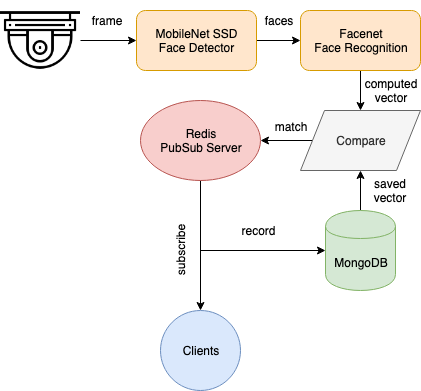
\includegraphics[scale=0.4]{gambar/sfa.png}
  % Keterangan gambar yang diinputkan
  \caption{Arsitektur Smart ITS Face Recognition System}
  % \citep{DiscoverySpaceShuttle}
  % Label referensi dari gambar yang diinputkan
  \label{fig:SpaceShuttle}
\end{figure}

\section{Implementasi Alat}

Pada implementasi Siffars kami mengimplementasikannya sebagai sistem absensi pegawai TU Departemen
Teknik Komputer ITS. Menggunakan CCTV/webcam sebagai input videonya siffars dapat mendeteksi kehadiran untuk
tiap-tiap pegawai berdasarkan kemiripan vector embeddings. Sebelumnya data wajah tiap-tiap pegawai harus
disimpan dalam database terlebih dahulu untuk dibandingkan dengan vector embeddings ketika siffars dijalankan.
Alur proses secara berurutan untuk penggunaan siffars sebagai sistem absensi adalah, Pertama menjalankan seluruh
aplikasi dan database yang digunakan untuk siffars, Kedua admin membuka halaman web untuk register/login jika sudah
pernah mendaftar sebelumnya, Ketiga admin memilih menu "add person" untuk menambahkan data wajah pegawai ke dalam database siffars
(semakin banyak data wajah semakin akurat), Keempat sistem akan otomatis mendeteksi wajah pegawai yang telah ditambahkan
dan nantinya akan ditampilkan ke web untuk waktu pegawai tersebut terdeteksi.


% Contoh pembuatan code snippet
% \begin{lstlisting}[
%   language=C++,
%   label={lst:Hello World},
%   caption={Program hello world}
% ]
% #include <iostream>

% int main() {
%     std::cout << "Hello World!";
%     return 0;
% }
% \end{lstlisting}

% % Contoh penggunaan referensi dari code snippet yang diinputkan
% Seperti contoh pada baris program Listing \ref{lst:Hello World} dan Listing \ref{lst:PrimeNumber}, \lipsum[23]

% % Contoh input code snippet
% \lstinputlisting[
%   % Bahasa yang digunakan oleh code snippet
%   language=Python,
%   % Label referensi dari code snippet yang diinputkan
%   label={lst:PrimeNumber},
%   % Keterangan dari code snippet yang diinputkan
%   caption={Program perhitungan bilangan prima}
% % Nama dari file code snippet yang diinputkan
% ]{program/prime-number.py}
